\documentclass[
    a4paper
]{scrreprt}
\usepackage[ngerman]{babel}
\usepackage[utf8]{inputenc}
\usepackage{textcomp, expdlist, array, colortbl, xcolor}
%\usepackage{wrapfig}
\usepackage[pdftex]{graphicx}
\usepackage[TS1, T1]{fontenc}
\usepackage{palatino} % Schriftart


\begin{document}
    \sffamily % Whole document sans-serif


    % Titelseite
    \begin{titlepage}
        \centering
        
\includegraphics[width=0.8\textwidth]{./images/logo_hska.png}\par\vspace{1cm}
        \vspace{1cm}

        {\scshape\Large Verteile Systeme 2 -- Labor\par}
        \vspace{1.5cm}

        {\huge\textbf{Twitter-Klon}\par}
        \vspace{2cm}

        {\Large\itshape Timo Blust, 48594\par}
        {\Large\itshape Gennadi Eirich, 50629\par}
        {\Large\itshape Tim Essig, 49683\par}
        {\Large\itshape Maike Rees, 47307\par}
        
        \vfill

        % Bottom of the page
        {\large \today\par}
    \end{titlepage}


    % Inhaltsverzeichnis
    \tableofcontents


    % Aufgabe 1
    \chapter{Konzeption und Gestaltung}
    \section{Use Case Diagramm}
    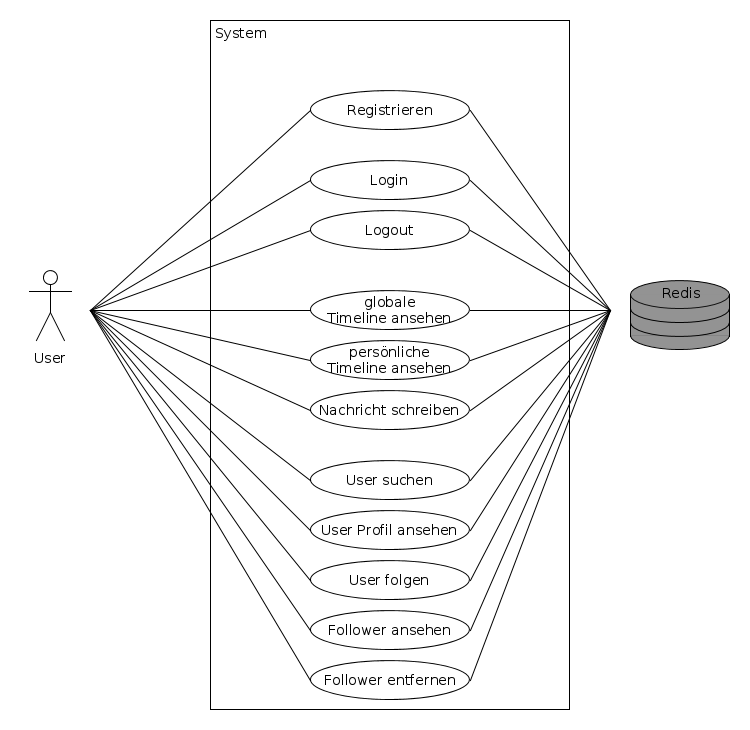
\includegraphics[width=\textwidth]{./images/useCaseDiagramm.png}
    \section{Entwurf der Seitennavigation}
    
    \section{Mockup}
    
    \section{Datenmodell}
    

    % Aufgabe 2
%    \chapter{Seitenbasierte Implementierung}


    % Aufgabe 3
%    \chapter{Asynchrone Erweiterungen}


\end{document}